\section{Graphical Representation}

\begin{figure}[H] % SSL Handshake
\center{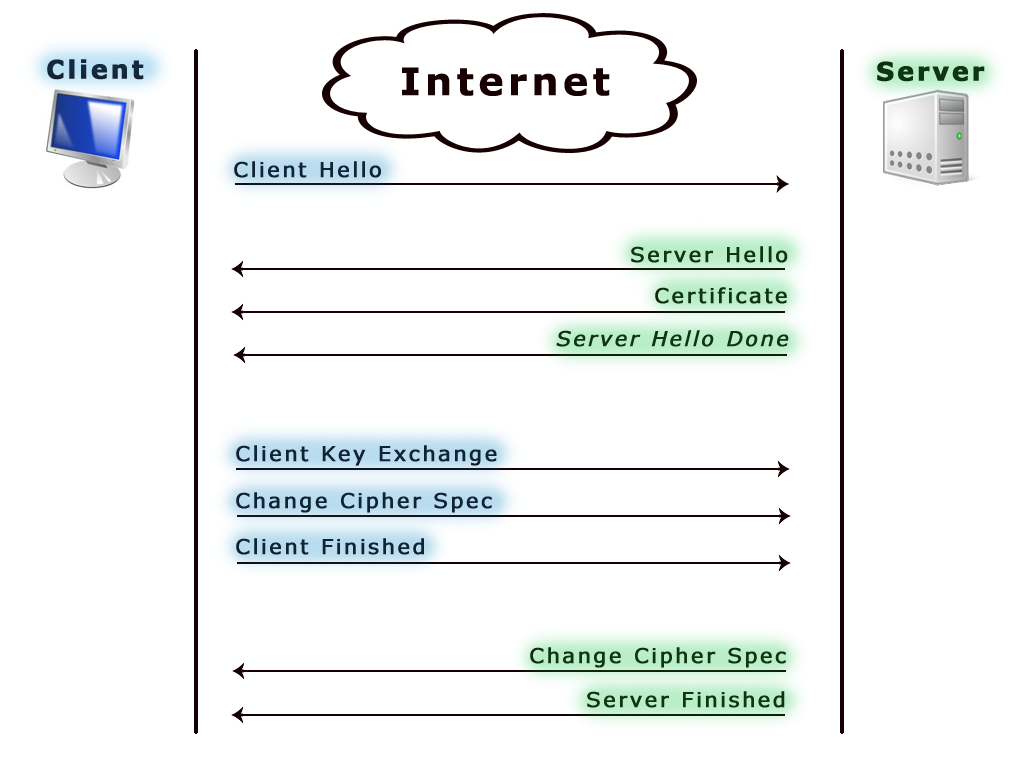
\includegraphics[width=1\linewidth]{SSL_handshake_image}}
\caption{SSL Handshake}
\label{fig:speciation}
\end{figure}

The graphic above shows how the SSL handshake is performed.

\begin{figure}[H] % SSL connection process
\center{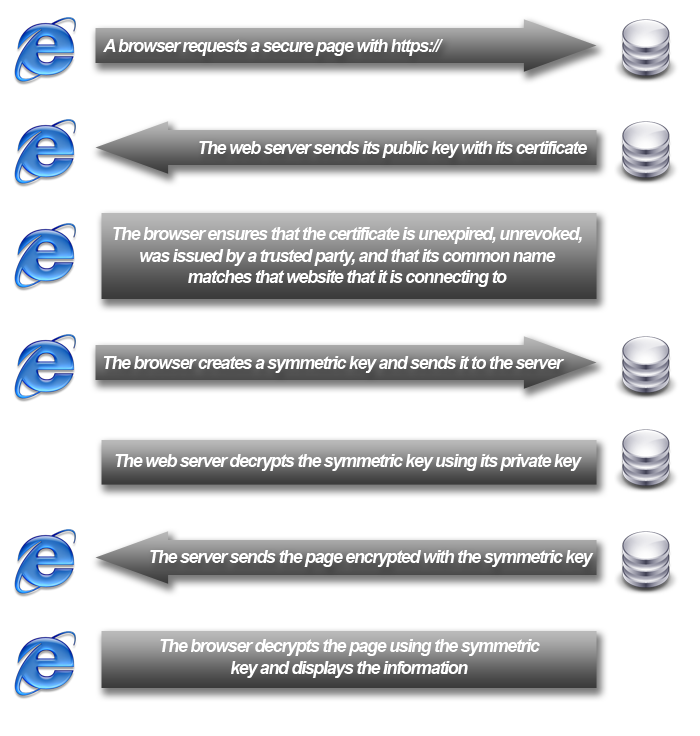
\includegraphics[width=1\linewidth]{what-is-ssl-connection-process}}
\caption{SSL connection process\cite{SSL_connection_process}}
\label{fig:speciation}
\end{figure}

The graphic above discribes the SSL connection process, and how the browser communicates with the server.

\begin{figure}[H] % Asymmetric encryption
\center{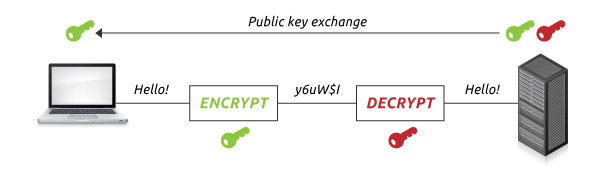
\includegraphics[width=0.8\linewidth]{Asymmetric_encryption}}
\caption{Asymmetric encryption\cite{Asymmetric_encryption}}
\label{fig:speciation}
\end{figure}

Graphical description of Asymmetric encryption in a very basic way.

\vspace{5mm}\hrule\vspace{5mm}

\begin{figure}[H] % symmetric encryption
\center{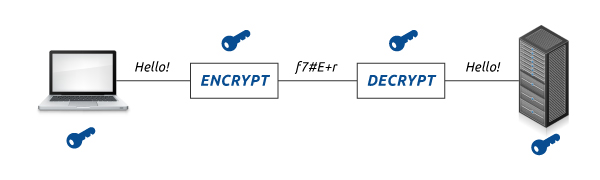
\includegraphics[width=0.8\linewidth]{symmetric_encryption}}
\caption{Symmetric encryption\cite{Symmetric_encryption}}
\label{fig:speciation}
\end{figure}

Graphical description of Symmetric encryption in a very basic way.

\begin{figure}[H] % PKI overview
\center{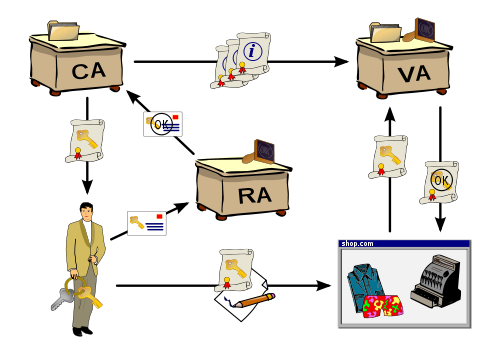
\includegraphics[width=0.8\linewidth]{pki-overview}}
\caption{PKI overview\cite{pki_overview}}
\label{fig:speciation}
\end{figure}

\vspace{5mm}\hrule\vspace{5mm}

This graphic shows an overview of a Public-key innfrastructure.

\begin{figure}[H] % Green bar overview
\center{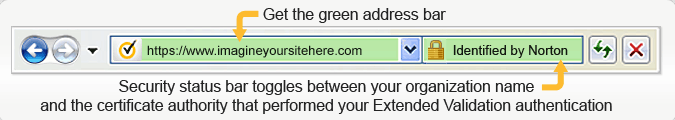
\includegraphics[width=1\linewidth]{green_bar}}
\caption{Green bar overview\cite{green_bar}}
\label{fig:speciation}
\end{figure}

This figure shows how some SSL certificates (often the highest trust-level) affects the users browser client.